\documentclass[11pt]{article}
\usepackage{fullpage}
\usepackage{amsthm}
\usepackage{amsmath}
\usepackage{amssymb}
\usepackage{graphicx}

\graphicspath{ {./imgs/} }

\setlength{\parindent}{0pt}

\title{Robotics (CO333)}
\author{Michael Tsang}

\newtheorem{defn}{Definition}
\newtheorem{eg}{Example}
\newtheorem{theo}{Theorem}
\newtheorem{lem}{Lemma}

\begin{document}

\maketitle

\section{Robot Motion}
A mobile robot can move and sense, and must process information to link these two.

What are the possible goals of a robot locomotion system?
\begin{itemize}
  \item Speed and/or acceleration of movement.
  \item Precision of positioning (repeatability).
  \item Flexibility and robustness in different conditions.
  \item Efficiency.
\end{itemize}

Robots could move in water, air, land, or even space.
We focus on wheeled robots which move on fairly flat surfaces.

\subsection{Motion and Coordinate Frames}
We define two coordinate frames: a \textbf{world frame} $W$ anchored in the world and a \textbf{robot frame} $R$ which is carried by and stays fixed relative to the robot at all times.

We are interested in the robot's \textbf{location}: the transformation between $W$ and $R$.

\subsection{Degrees of Motion Freedom}
A rigid body which translates and rotates along a:
\begin{itemize}
  \item 1D path has 1 degree of freedom (DOF): 1 translational.
  \item 2D plane has 3 DOF: 2 translational, 1 rotational.
  \item 3D volume has 6 DOF: 3 translational, 3 rotational.
\end{itemize}

A \textbf{holonomic robot} is one which is able to move instantaneously in any direction in the space of its degrees of freedom.

Although holonomic robots exist, they need many motors or unusual designs, and are often impractical.

\subsection{Wheel Configurations}
\begin{itemize}
  \item Rack and Pinion.
  \item Differential Drive.
  \item Skid-Steer.
  \item Synchro Drive.
\end{itemize}
These are standard non-holonomic configurations and are simple, reliable, robust mechanisms suitable for robots which essentially move in a plane.

Some more exotic non-holonomic configurations are:
\begin{itemize}
  \item Segway - good height with small footprint and high acceleration; self balancing.
  \item Mars Rover - wheels on stalks to tackle large obstacles.
\end{itemize}

\subsection{Differential Drive}
\begin{itemize}
  \item Two motors, one per wheel.
  \item Steer by setting different speeds on each wheel.
  \item Wheels run at equal speeds for straight-line motion.
  \item Wheels run at equal and opposite speeds to turn on the spot.
  \item Other combinations of speeds allow circular arcs.
\end{itemize}

\subsection{Circular Path of a Differential Drive Robot}
\begin{figure}[h]
  \caption{Differential Drive Robot}
  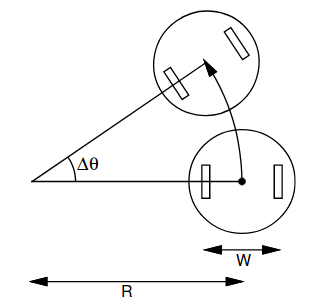
\includegraphics[scale=0.4]{ddrobot}
  \centering
\end{figure}

Let the wheel velocities of the left and right wheels respectively be $v_L$ and $v_R$.
These are linear velocities of the wheels over the ground: $v_X = r_X\omega_X$, where $r_X$ is the radius of the $X$ wheel and $\omega_X$ is its angular velocity.

The width between the wheels is $W$.

\begin{itemize}
  \item Straight line motion if $v_L = v_R$.
  \item Turns on the spot if $v_L = - v_R$.
\end{itemize}

To find radius $R$ of a curved path, consider a period of motion $\Delta t$ where the robot moves along a circular arc through angle $\Delta \theta$.
\begin{itemize}
  \item Left wheel: $\text{distance moved } = v_L \Delta t$; $\text{radius of arc } = R - \frac{W}{2}$.
  \item Right wheel: $\text{distance moved } = v_R \Delta t$; $\text{radius of arc } = R + \frac{W}{2}$.
  \item Both wheel arcs subtend the same angle so:
    \[
      \Delta \theta = \frac{v_L \Delta t}{R - \frac{W}{2}} = \frac{v_R \Delta t}{R + \frac{W}{2}}
    \]
    \[
      \implies \frac{W}{2}(v_L + v_R) = R(v_R - v_L)
    \]
    \begin{align*}
      \implies R &= \frac{W(v_R + v_L)}{2(v_R - v_L)} & \Delta \theta &= \frac{(v_R - v_L)\Delta t}{W}
    \end{align*}
\end{itemize}

\subsection{Rack and Pinion Drive (Car/Tricycle)}
\begin{figure}[h]
  \caption{Rack and Pinion Drive layouts.}
  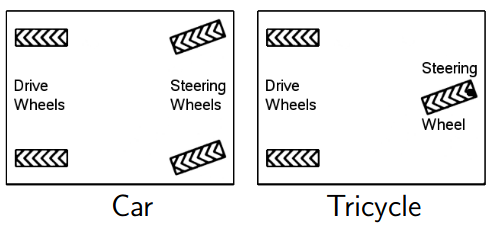
\includegraphics[scale=0.4]{piniondrive}
  \centering
\end{figure}

\begin{itemize}
  \item Two motors: one to drive, one to steer.
  \item Cannot normally turn on the spot.
  \item With fixed speed and steering angle, will follow a circular path.
  \item With four wheels, need rear differential and variable (``Ackerman'') linkage for steering wheels.
\end{itemize}

\subsection{Circular Path of a Car-Like Tricycle Robot}
\begin{figure}[h]
  \caption{Tricycle Robot.}
  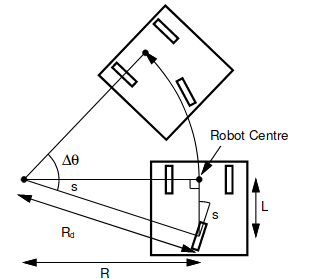
\includegraphics[scale=0.5]{tricycle}
  \centering
\end{figure}

Single steerable and drivable wheel at back, front wheels are free running.

Assuming no sideways wheel slip, we intersect the axes of the front and back wheels to forma right-angle triangle:
\[
  R = \frac{L}{\tan s}
\]

The radius of the path the rear wheels moves is:
\[
  R_d = \frac{L}{\sin s}
\]

In time $\Delta t$, the distance along its circular arc moved by the wheel is $v\Delta t$, so the angle $\Delta \theta$ through which the robot rotates is:
\[
  \Delta \theta = \frac{v\Delta t}{R_d} = \frac{v\Delta t \sin s}{L}
\]

\subsection{Gearing}
\begin{figure}[h]
  \caption{Gears of a DC motor.}
  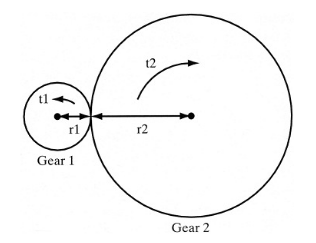
\includegraphics[scale=0.5]{gearing}
  \centering
\end{figure}

DC motors offer high speed and low torque, so gearing is nearly always required to drive a robot.

If Gear 1 is driven with torque $t_1$, it exerts tangential force:
\[
  F = \frac{t_1}{r_1}
\]

on Gear 2; the torque in Gear 2 is therefore:
\[
  t_2 = r_2F = \frac{r_2}{r_1}t_1
\]

The change in angular velocity between Gear 1 and Gear 2 is calcualted by considering velocity at the point where they meet:
\[
  v = \omega_1 r_1 = \omega_2 r_2
\]
\[
  \implies \omega_2 = \frac{r_1}{r_2}\omega_1
\]
\begin{itemize}
  \item When a small gear drives a bigger gear, the second gear has higher torque and lower angular velocity in proportion to the ratio of teeth.
  \item Gears can be chained together to achieve compound effects.
\end{itemize}

\subsection{Motor Control - Open Loop}
\begin{figure}[h]
  \caption{Open loop system.}
  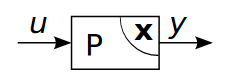
\includegraphics[scale=0.4]{openloop}
  \centering
\end{figure}

Let $P$ be a Single-Input-Single-Output (SISO) dynamic system, it is described by:
\begin{itemize}
  \item An input $u$ - here: voltage $V$, or corresponding Pulse Width Modulation (PWM) value.
  \item Internal states $x$, whose dynamics follow differential equations - here: $x = [x_1, x_2]^\top = [\omega, \varphi]^\top$, with rotation speed $\omega$ and angle $\varphi$.
  \item An output $y$ as a function of $x$ - here: angle $\varphi$, $y = x_2$.
\end{itemize}

Qualitative open-loop response on input (voltage) step: input $V$ leads to output motor angle $\phi$, which changes with time.

\subsection{Motor Control - Closed Loop}
\begin{figure}[h]
  \caption{Closed loop system.}
  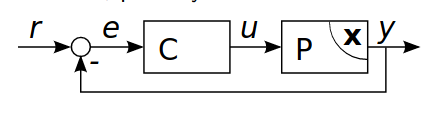
\includegraphics[scale=0.4]{closedloop}
  \centering
\end{figure}

Let $C$ be a controller possibly with internal states:
\begin{itemize}
  \item $r$ is a reference (desired) output.
  \item $e$ is the e  rror between reference and actual output.
\end{itemize}

The controller runs at a high frequency, at each iteration it checks the current error and calculates a control value to the motor which aims to reduce the error.

This is simple: a binary on or off.

\subsection{General Motor Control - PID}
Proportional-Integral-Differential (PID), a controller:
\[
  C : u(t) = k_p \exp(t) + k_i \int_{t_0}^{t} \exp(\tau)d_\tau + k_d \frac{d\exp(t)}{dt}
\]
where
\begin{itemize}
  \item $k_p$ - proportional gain, reduces the error.
  \item $k_i$ - integral gain, removes steady-state error.
  \item $k_d$ - differential gain, can reduce settling time.
\end{itemize}

A simple (heuristic) tuning rule is the \textbf{Ziegler-Nichols}:
\begin{itemize}
  \item Set $k_i$ and $k_d$ to zero.
  \item Increase $k_p$ until the system starts oscillating with Period $P_u$ (in seconds) - remember this gain as $k_u$.
  \item Set $k_p = 0.6k_u, k_i = 2k_p/P_u, \text{and } k_d = k_pP_u/8$.
\end{itemize}

\subsection{Motor Control - Additional Tweaks}
\begin{itemize}
  \item Reference filtering - respect physical limits already in reference.
  \item Anti-Reset-Windup - stops integrating the effor for the I-part, when $u$ is at its physical limit.
  \item Dead-band compensation - add offset to $u$ to compensate friction.
  \item Feed-forward controller - $C_f : u_f(t) = k_f \frac{dr(t)}{dt}$, reduces ``work'' for the feedback controller
\end{itemize}

\subsection{Mapping Wheel Rotation Speed to Velocity}
In principle, we could emasure the radius of each wheel $r_W$ to turn angular into linear motion.
However in practice, due to hard to model factors, it is better to calibrate empirically, i.e.\ work out the scaling between the motor reference angle and the distance travelled over the ground via experiments.

\subsection{Motion and State on a 2D Plane}
We can define a \textbf{state vector} $\textbf{x}$:
\[
  \textbf{x} = 
  \begin{pmatrix}
    x \\ y \\ \theta
  \end{pmatrix}
\]
\begin{itemize}
  \item $x$ and $y$ specify the location of the pre-define ``robot centre'' point in the world frame.
  \item $\theta$ specifies the rotation angle between the two coordinate frames (the angle between the $x^W$ and $x^R$ axes).
  \item At the origin, $x = y = \theta = 0$.
\end{itemize}

\subsection{Integrating Motion in 2D}
2D motion on a plane: three degrees of position freedom $(x, y, \theta)$, with $-\pi < \theta \leq \pi$.

Consider a robot which either drives ahead or turns on the spot:
\begin{itemize}
  \item During straight-line period of motion of distance $D$:
    \[
      \begin{pmatrix}
        x_{\text{new}} \\
        y_{\text{new}} \\
        \theta_{\text{new}} 
      \end{pmatrix}
      =
      \begin{pmatrix}
        x + D\cos\theta \\
        y + D\sin\theta \\
        \theta 
      \end{pmatrix}
    \]
  \item During a pure rotation of angle $\alpha$:
    \[
      \begin{pmatrix}
        x_{\text{new}} \\
        y_{\text{new}} \\
        \theta_{\text{new}} 
      \end{pmatrix}
      =
      \begin{pmatrix}
        x \\
        y \\
        \theta + \alpha
      \end{pmatrix}
    \]
\end{itemize}

\subsection{Integrating Circular Motion Estimates in 2D}
\begin{figure}[h]
  \caption{Circular Motion estimation.}
  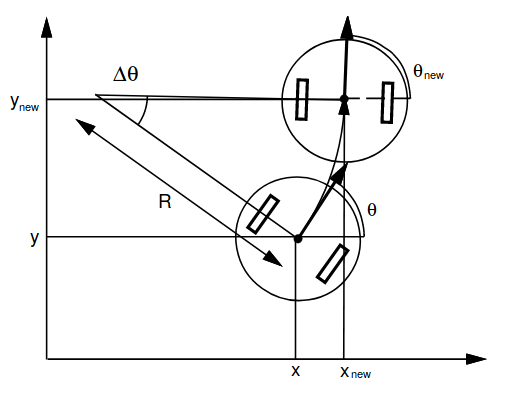
\includegraphics[scale=0.4]{circularmotionestimate}
  \centering
\end{figure}

\[
  \begin{pmatrix}
    x_{\text{new}} \\
    y_{\text{new}} \\
    \theta_{\text{new}} 
  \end{pmatrix}
  =
  \begin{pmatrix}
    x + R(\sin(\Delta \theta + \theta) - \sin \theta) \\
    y - R(\cos(\Delta \theta + \theta) - \cos \theta) \\
    \theta + \Delta \theta
  \end{pmatrix}
\]

\subsection{Position-Based Path Planning}
Assuming that robot has localisation and knows where it is relative to a fixed coordinate frame, then \textbf{position-based path planning} allows it to move in precise way along a sequence of pre-defined waypoints.
Paths of various curved shapes could be planning, aiming to optimise criteria (e.g.\ time or power).

We assume that:
\begin{itemize}
  \item Movements are composed by straight-line segments separated by turns on the spot.
  \item Total distance travelled is minimised - it always faces to turn the next waypoint and drive straight towards it.
\end{itemize}

If the current pose is $(x, y, \theta)$ and the next waypoint is $(W_x, W_y)$, it must first rotate to point towards the waypoint at vector direction:
\[
  \begin{pmatrix}
    d_x \\
    d_y
  \end{pmatrix}
  =
  \begin{pmatrix}
    W_x - x \\
    W_y - y
  \end{pmatrix}
\]
The absolute angular orientation $\alpha$ the robot must drive in is:
\[
  \alpha = \tan^{-1} \frac{d_x}{d_y}
\]

Care must be taken to ensure $\alpha$ is in the correct quadrant of $-\pi < \alpha \leq \pi$.

The angle the robot must rotate through is therefore $\beta = \alpha - \theta$.
To move as efficiently as possible, care should be taken to shift this angle by adding or subtracting $2\pi$ to ensure $-\pi < \beta \leq \pi$.

The robot should then drive forward straight for
\[
  d = \sqrt{d_x^2 + d_y^2}
\]

\end{document}

